\chapter{Batching Operations for Isogenies}

Our first contribution to the \sidh codebase is the implementation and integration of a procedure for batching together many $\mathbb{F}_{p^2}$ element inversions. This contribution is discussed in detail in the following chapter. The chapter is split into three sections: a high-level discussion of the procedure itself, the low-level details of its integration into \sidh, and finally, the resulting affects of this procedure on the performance of \sidh. 

In the first section of this chapter we will detail the specifics of the partial batched inversion procedure. We will show how the procedure can be constructed by combining two techniques: a well known method for reducing a $\mathbb{F}_{p^2}$ inversion to several $\mathbb{F}_{p}$ operations, and an inversion batching technique outlined in \cite{batching}. 

As we then venture into the lower-level implementation details, we will explore how the procedure can be leveraged optimally in the codebase. We will take a closer look at several of the aforementioned \sidh functions as we illustrate some of the performance bottlenecks in the system. At this time, we will also discuss the design decisions made while implementing the partial batched inversion procedure as well as some of the functions lower-level minutiae.

We will end this chapter by taking a detailed look at the performance gains offered by the inclusion of partial batched inversions in \sidh. More precisely, we will be examining the effects of the procedure on the Yoo et al. signature layer. We will contrast the measured performance of our implementation with an analytical calculation of the expected improvement, and discuss the possible origins of divergent behaviour.  

\section{Partial Batched Inversions}

We will now outline our first contribution to \sidh. The ``partial batched inversion" procedure in question reduces arbitrarily many \emph{unrelated} $\mathbb{F}_{p^{2}}$ inversions to a sequence of $\mathbb{F}_{p}$ operations. The fact that the elements being inverted need not hold any relation will be significant to the applicability of this procedure. For brevities sake, we will henceforth refer to this procedure as \code{pb\_inv} in the \sidh context, and \textbf{PartialBatchedInversion} in the more general mathematical context.

As mentioned above, \code{pb\_inv} is constructed by combining two distinct techniques. Both of these techniques improve the efficiency of computing field element inversions: the first is specific to extension fields (in our case, $\mathbb{F}_{p^{2}}$ elements,) but the second is a technique applicable to field element inversions in a more general setting.

We will begin with a dissection of these two techniques, starting first with the ``partial" inversion technique and then looking at batched inversions. The definitions we will give for these techniques below are given at the level of field arithmetic. When we proceed to sketch \code{pb\_inv}, we will offer two definitions: one in this section given at the abstraction-level of field arithmetic, and one in the proceeding section given in terms of \sidh syntax.

In the subsections to come, when we are working at the level of field arithmetic we will denote the first and second portions of an arbitrary $x \in \mathbb{F}_{p^{2}}$ as $x_{a}$ and $x_{b}$ respectively. We identify $x$ by saying $x = \{x_{a}, x_{b}\}$. Recall from \ref{subsec:fields} that both $x_{a}$ and $x_{b}$ are valid $\mathbb{F}_{p}$ elements. 

We will express the performance of the comming procedures in terms of the sum number of underlying field operations within them. We denote the computation time for base field arithmetic with bold letters (such as \textbf{a} for $\mathbb{F}_p$ \textbf{a}ddition), and we use bold letters accented with a ``closure" bar for extension field arithmetic ($\bar{\textbf{a}}$ for $\mathbb{F}_{p^2}$ \textbf{a}ddition). For example, the performance of some procedure $P$, which we might write as $C_{P}$, may look like the following:
$$
C_{P} = 2\bar{\textbf{a}} + x\bar{\textbf{i}} + y\textbf{m} + \textbf{s}
$$
Which denotes that $P$ is a procedure composed of 2 $\mathbb{F}_{p^{2}}$ additions, $x$-many $\mathbb{F}_{p^{2}}$ inversions, $y$-many $\mathbb{F}_{p}$ multiplications, and a single $\mathbb{F}_{p}$ squaring. We reserve uppercase bold letters for arithmetic over elliptic curve points (such as \textbf{A} to denote the point-wise addition operation).

\subsection{$\mathbb{F}_{p^{2}}$ Inversions done in $\mathbb{F}_{p}$}

There is a simple way in which we can perform one $\mathbb{F}_{p^{2}}$ inversion by means of doing several $\mathbb{F}_{p}$ operations. We will begin by considering multiplicative inverses of complex numbers. Fields of the form $\mathbb{F}_{q^{2}}$ for some prime $q$ are, after all, quadratic extension fields; because of this $\mathbb{F}_{p^{2}}$ arithmetic is treated, for the most part, analogously to complex number arithmetic.

Consider the complex number $C = a + bi$. We have that $C^{-1} = 1 / (a + bi)$, from which we can rationalize the denominator like so:\\
$$
C^{-1} = \frac {1}{(a + bi)} \cdot \frac{(a - bi)}{(a - bi)}
$$
$$
C^{-1} = \frac {a - bi}{(a + bi)(a - bi)}
$$
Here we note that $(a + bi)(a - bi)$ is equivalently $(a^2 - b^2)$ and so we can rewrite $C^{-1}$ as the following:
$$
C^{-1} = \frac {a - bi}{(a)^2 - (bi)^2}
$$
$$
C^{-1} = \frac {a - bi}{a^2 + b^2}.
$$

Elements in the quadratic extension of a finite field are treated similarly, such that if we take some element $x = \{x_{a}, x_{b}\} \in \mathbb{F}_{p^{2}}$ for some prime $p$, we can equivalently represent $x$ as $x_{a} + x_{b}i$ and treat arithmetic on $x$ exactly as we would for a complex number (modulo $p$, of course). From this we can see that $x^{-1}$ can be defined as:
$$
x^{-1} = \{\frac {x_{a}}{x_{a}^2 + x_{b}^2}, \frac {-x_{b}}{x_{a}^2 + x_{b}^2}\}
$$

Now it is clear that we can compute the multiplicative inverse of $x$ by computing: the inverse of $x_{a}^2 + x_{b}^2$, which is of course an inversion in $\mathbb{F}_{p}$, and $-x_{b}$, which is a relatively inexpensive operation (also in the base field). Below, we formulate this technique as algorithm \ref{alg:partialinv}, which we refer to as \textbf{PartialInv}.\\

\begin{algorithm}[!h]
\caption{-- \textbf{PartialInv($x \in \mathbb{F}_{p^{2}}$)}}\label{alg:partialinv}
\begin{algorithmic}[1]
\State $den \gets x_{a}^{2} + x_{b}^{2}$

\State $den_{inv} \gets den^{-1}$

\State $a \gets x_{a} \cdot den_{inv}$

\State $b \gets -(x_{b}) \cdot den_{inv}$

\State $x^{-1} \gets \{a, b\}$

\State \Return $x^{-1}$
\end{algorithmic}
\end{algorithm}

Effectively, this procedure reduces one $\mathbb{F}_{p^{2}}$ inversion to the following operations: 

\begin{center}
\begin{itemize}
\item 2 $\mathbb{F}_{p}$ squarings -- \emph{line 1 of algorithm} \ref{alg:partialinv}
\item 1 $\mathbb{F}_{p}$ addition -- \emph{line 1 of algorithm} \ref{alg:partialinv}
\item 1 $\mathbb{F}_{p}$ inversion -- \emph{line 2 of algorithm} \ref{alg:partialinv}
\item 3 $\mathbb{F}_{p}$ multiplications -- \emph{lines 3 \& 4 of algorithm} \ref{alg:partialinv}
\end{itemize}
\end{center}

We say ``reduces", but it may not be immediately clear that this technique is computationally favourable over any other approach to computing an $\mathbb{F}_{p^{2}}$ inversion. 

\subsection{Batching Field Element Inversions}

The second technique used in the composition of \code{pb\_inv} reduces arbitrarily many (general) field element inversions to \emph{one} inversion and a linearly scaling amount of multiplcations in the \emph{same} field.

This technique was outlined by Shacham and Boneh in \cite{batching}. Shacham and Boneh provided several techniques for improving the performance of SSL handshakes, most of which built on the earlier efforts of Amos Fiat in batching multiple RSA decryptions. While somewhat related, Fiat's work admittedly is only applicable to the RSA cryptosystem, and requires additional constraints on the elements being batched. 

One improvement offered by Shacham and Boneh, however, is their proposed notion of batching together divisions from across multiple unrelated SSL instances. 

Suppose we want to compute the inverses of three elements $x, y, z \in F$ where $F$ is some arbitrary field. The batched division technique allows us to reduce these three inversions to one. The technique can be organized into three phases. In the first phase, all the elements of the batch are multiplied together into one product, yielding $a = xyz$. We refer to this first phase as ``upward-percolation". Next, we compute the inverse of $a$: $a^{-1} = (xyz)^{-1}$, which we refer to as the inversion phase. In the final phase, ``downward-percolation", we can compute each individual element's multiplicative inverse as follows:
$$
x^{-1} = a^{-1} \cdot (yz)
$$
$$
y^{-1} = a^{-1} \cdot (xz)
$$
$$
z^{-1} = a^{-1} \cdot (xy)
$$

Let us analyse these phases a little more closely while we generalize to $n$-many elements. In the upward-percolation phase, constructing $a$ requires $n-1$ multiplications; and so has a complexity of $\mathcal{O}(n)$. The inversion phase requires one field element inversion, and so has complexity of $\mathcal{O}(1)$. 

If we implement the downward-percolation phase directly as outlined in the three-element example above, computing every output requires $n$ products each composed of $n-1$ multiplications. These $n$ products are each also multiplied by $a^{-1}$. This multiplication by $a^{-1}$ can be added to our $n-1$ inversion count resulting in $n$-many products composed of $n$ multiplications; bringing the complixity of the downward-percolation phase to $\mathcal{O}(n^2)$.

Let $B_0$ denote the performance of the approach above to batching field element inversions. We have, then, that 
$$
B_0 = n^2\bar{\textbf{m}} + (n-1)\bar{\textbf{m}} + \bar{\textbf{i}}.
$$\\

\noindent
This batching proceedure can be thought of as analogous to traditional time-memory tradeoff algorithms. In a general time-memory tradeoff algorithm you can continue to make some linear or polynomial (or otherwise) sacrifice of memory in order to gain some increase in performance. In the batching procedure described above we are in some sense sacrificing some marginal amount of memory to gain an increase in performance, but it is not a tradeoff that we can adjust to our liking.

There is a way, much akin to this time-memory tradeoff strategy, that we can further reduce the execution time of this procedure. In the upward-percolation phase, we currently store in $a$ the product of elements $x_0 \cdot x_1 \cdot ... \cdot x_{n-1}$. Suppose instead that we store in $a$ an \emph{array} (size $n$) of elements, defined in the following way:
$$
a_i = 
\begin{cases}
x_0 & i = 0\\
a_{i-1} \cdot x_i & \text{otherwise}
\end{cases}
$$
Equivalently, the elements of this array are
$$
a_0 = x_0, \quad a_1 = x_0 \cdot x_1, \quad a_2 = x_0 \cdot x_1 \cdot x_2, \quad ... 
$$
and so on and so forth up to $n-1$. In the inversion phase we will compute $inv = a_{n-1}^{-1}$; we are still inverting the product of all the elements, but because we have stored the value of the product at every step of the way, we can save on a significant number of operations in the downward-percolation phase.

Going into the final stage of the procedure now, we can compute $x_{n-1}^{-1}$ simply by computing $inv \cdot a_{n-2}$. Moving forward (or backwards, technically), we peel the previously used $x_{n-1}^{-1}$ off of $inv$ by computing $inv := inv \cdot x_{n-1}$ and, with our updated $inv$, we compute $x_{n-2}^{-1} = inv \cdot a_{n-3}$. We proceed in this fashion until we reach $x_{0}^{-1}$, which (if we've been updating $inv$ every step of the way) is simply equal to $inv$. 

We provide an algorithm under the name of \textbf{BatchedInv} implementing this approach, generalized to $n$-many elements (See Algorithm \ref{alg:batchedinv}). In Algorithm \ref{alg:batchedinv}, lines 1--3 implement the upward-percolation phase. Line 4 carries out the second phase: the inversion of $a_{n-1}$. The third and final stage, downward-percolation, occurs from lines 5 to 7.

\begin{algorithm}
\caption{-- \textbf{BatchedInv($\{x_0, x_1, ..., x_n-1\} \in \mathbb{F}_{p^{2}}^{n}$)}}\label{alg:batchedinv}
\begin{algorithmic}[1]
\State $a_0 \gets x_0$

\For{\texttt{i = 1..(n-1)}}
	\State $a_i \gets a_{i-1} \cdot x_i$
\EndFor

\State $inv \gets a_{n-1}^{-1}$

\For{\texttt{i = (n-1)..1}}
	\State $x_i^{-1} \gets a_{i-1} \cdot inv$
	\State $inv \gets inv \cdot x_{i}$
\EndFor

\State $x_0^{-1} = inv$

\end{algorithmic}
\end{algorithm}

\textbf{BatchedInv} can be used to reduce $n$-many $\mathbb{F}_{p^{2}}$ inversions to the following operations:

\begin{center}
\begin{itemize}
\item $n-1$ $\mathbb{F}_{p^2}$ multiplications -- \emph{line 2-3 of algorithm} \ref{alg:batchedinv}
\item 1 $\mathbb{F}_{p^2}$ inversion -- \emph{line 4 of algorithm} \ref{alg:batchedinv}
\item $2(n-1)$ $\mathbb{F}_{p^2}$ multiplications -- \emph{line 5-7 of algorithm} \ref{alg:batchedinv}
\end{itemize}
\end{center}

\noindent
Let $B$ denote the performance of \textbf{BatchedInv}. 
$$
B = 2(n-1)\bar{\textbf{m}} + (n-1)\bar{\textbf{m}} + \bar{\textbf{i}}.
$$

Comparing the performance of \textbf{BatchedInv} with our initial construction, we see that $B < B_0$ holds when the following holds:
$$
2(n-1)\bar{\textbf{m}} + (n-1)\bar{\textbf{m}} + \bar{\textbf{i}} < n^2\bar{\textbf{m}} + (n-1)\bar{\textbf{m}} + \bar{\textbf{i}}
$$
$$
2(n-1)\bar{\textbf{m}} < n^2\bar{\textbf{m}}
$$
$$
2(n-1) < n^2
$$


And so \textbf{BatchedInv} outperforms our original roughly-sketched procedure when the number of elements being batched ($n$) exceeds 2.

\subsection{Partial Batched Inversions}

We have now outlined the following: \textbf{PartialInv} as a technique for computing $\mathbb{F}_{p^2}$ inversions by means of $\mathbb{F}_{p}$ arithmetic, and \textbf{BatchedInv} as a technique for batching together arbitrarily many inversion operations. We will now combine these procedures in a (near) trivial manner to achieve the partial batched inversion algorithm.

At first glance, an attempt to meld these two techniques together might be made in the following way:

\begin{algorithm}
\caption{-- \textbf{PartialBatchedInvAttempt($\{x_0, x_1, ... , x_{n-1}\}$)}}\label{alg:partialinv}
\begin{algorithmic}[1]
\State $a \gets$ upward-percolation of elements $\{x_0, x_1, ... , x_{n-1}\}$

\State $a^{-1} \gets$ \textbf{PartialInv($a$)}

\State $\{x_{0}^{-1}, x_{1}^{-1}, ... , x_{n-1}^{-1}\} \gets$ downward-percolation of $a^{-1}$

\State \Return $\{x_{0}^{-1}, x_{1}^{-1}, ... , x_{n-1}^{-1}\}$
\end{algorithmic}
\end{algorithm}
\noindent
Counting the sum of operations in this proposed approach, we have the following: 
\begin{itemize}
\item $n$ $\mathbb{F}_{p^2}$ multiplications -- \emph{upward-percolation phase}
\item 2 $\mathbb{F}_{p}$ squarings, 1 $\mathbb{F}_{p}$ addition, 1 $\mathbb{F}_{p}$ inversion, and 3 $\mathbb{F}_{p}$ multiplications -- \emph{call to} \textbf{PartialInv($a$)}
\item $2n$ $\mathbb{F}_{p^2}$ multiplications -- \emph{downward-percolation phase}
\end{itemize}
To measure the complixity in terms of field operations, denoted $C'$, we can surmize the the total operation count as:
$$
C' = (n\bar{\textbf{m}}) + (2\textbf{s} + \textbf{a} + \textbf{i} + 3\textbf{m}) + (2n\bar{\textbf{m}})
$$
$$
C' = 3n\bar{\textbf{m}} + 2\textbf{s} + \textbf{a} + \textbf{i} + 3\textbf{m}
$$

Below we provide an alternative approach to building \textbf{PartialBatchedInv} that relies on only $\mathbb{F}_{p}$ operations. Afterward, we show by simply analysis why this approach yields the better performance. This procedure is formalized in a mathematical setting in algorithm \ref{alg:pbinvmath}. We give a precise C function definition in section \ref{sec:pbinvimplementation}.

\begin{algorithm}
\caption{-- \textbf{PartialBatchedInversion($\mathbb{F}_{p^{2}}$ $\{x_0, x_1, ..., x_n-1\}$)}}\label{alg:pbinvmath}
\begin{algorithmic}[1]
\Procedure{partial\_batched\_inv($\mathbb{F}_{p^{2}}$[ ] vec, $\mathbb{F}_{p^{2}}$[ ] dest, int n)}{}
\For{\code{i = 0..(n-1)}}
	\State $den_{i} \gets (x_i)_{a}^{2} + (x_i)_{b}^{2}$
\EndFor

\State $a_0 \gets den_0$

\For{\code{i = 1..(n-1)}}
	\State $a_i \gets a_{i-1} \cdot den_i$
\EndFor

\State $inv \gets inv(a_{n-1})$

\For{\code{i = n-1..1}}
	\State $a_i \gets inv \cdot dest_{i-1}$
	\State $inv \gets inv \cdot den_i$
\EndFor

\State $a_0 \gets a_{inv}$

\For{\code{i = 0..(n-1)}}
	\State $(xinv_i)_a \gets a_i \cdot (x_i)_a$
	\State $(xinv_i)_b \gets a_i \cdot -(x_i)_b$
	\State $x_i^{-1} \gets \{(xinv_i)_a, (xinv_i)_b\}$
\EndFor
\State \Return $\{x_0^{-1}, x_1^{-1}, ..., x_n-1^{-1}\}$
\EndProcedure
\end{algorithmic}
\end{algorithm}
\noindent

$a$ is a simple auxillary set we use to hold the inverted $\mathbb{F}_{p}$ elements. After these are all computed via the for-loop on line 8, we can reconstruct $\mathbb{F}_{p}$

More specifically, the procedure takes us from $n$ $\mathbb{F}_{p^{2}}$  inversions to: 
\begin{center}
\begin{itemize}
\item 2\textit{n} $\mathbb{F}_{p}$ squarings
\item \textit{n} $\mathbb{F}_{p}$ additions
\item 1 $\mathbb{F}_{p}$ inversion
\item 3(\textit{n}-1) $\mathbb{F}_{p}$ multiplications
\item 2\textit{n} $\mathbb{F}_{p}$ multiplications
\end{itemize}
\end{center}
\noindent
And so, with $C$ measuring the performance of \textbf{PartialBatchedInversion}, we have
$$
C = 2n\textbf{s} + n\textbf{a} + \textbf{i} + 3(n-1)\textbf{m} + 2n\textbf{m}
$$
We can further simplify $C$ if we presume that a the execution time of squaring is roughly the same as multiplication. Additionally, we can simplify $3(n-1)$ to $3n$ in the spirit of complexitiy theory. With these simplifications we arrive at
$$
C \approx 7n\textbf{m} + n\textbf{a} + \textbf{i}
$$
Applying the same simplifying assumptions to $C'$, we arrive at
$$
C' \approx 3n\bar{\textbf{m}} + 5\textbf{m} + \textbf{a} + \textbf{i} 
$$
We note here that an $\mathbb{F}_{p^2}$ multiplication (\textbf{M}) is performed simply by means of 4 $\mathbb{F}_{p}$ multiplications (again, recall the multiplcation of complex numbers). So we have $\textbf{M} = 4\textbf{m}$, and can further simplify $C'$:
$$
C' \approx (12n + 5)\textbf{m} + \textbf{a} + \textbf{i}
$$
Finally we've simplified $C$ and $C'$ to forms that are more easily compared. Let $\textbf{P}$ denote the proposition that $C$ runs in fewer operations than $C'$:
$$
\textbf{P} \equiv C < C'
$$
$$
\textbf{P} \equiv 7n\textbf{m} + n\textbf{a} + \textbf{i} < (12n + 5)\textbf{m} + \textbf{a} + \textbf{i}
$$
Simplifying slightly, we need now to resolve
$$
7n\textbf{m} + n\textbf{a} < (12n + 5)\textbf{m} + \textbf{a}
$$

\subsection{Applicability to \sidh}

Because the work of Yoo et al. was built on top of the original Microsoft SIDH library, all underlying field arithmetic (and as such, pointwise arithmetic) is performed in projective space using Montgomery representation. As was mentioned in the previous chapter, doing such allows us to avoid a great deal of field element inversions. We simply convert to Montgomery representation at the beginning of heavy arithmetic, perform the desired operations, and then convert back to standard representation when complete. Throughout the codebase, (most noticeably in \code{kex.c}) we can see an analogous approach taken in for pointwise arithmetic, by first converting to a projective space representation, performing operations, and then converting back to affine coordinates. 

 The downside of this (for our work) is that the number opportunities for implementing the batched inversion algorithm becomes greatly limited.\\

\section{Implementation Details}
\label{sec:pbinvimplementation}

We will now take the work of the previous section and explain in detail how it can be applied to the Yoo et al. signature layer of \sidh. We begin first by transcribing \textbf{PartialBatchedInversion} to its programmatic variant, \code{pb\_inv}. In the subsections to come, we offer explainations for some of the design choices made in the implementation of \code{pb\_inv}, both at a micro level (algorithmic details of the procedure) and a macro level (specifics of implementation within \sidh).

With Algorithm \ref{alg:pbinvcode} we provide an explicit C definition for the function \code{pb\_inv}. For descriptions of the functions called in this procedure, the reader can refer to section \ref{subsec:functions}. For explicit definitions of some of these functions, the reader can refer to appendix [insert appendix].

\begin{algorithm}
\caption{-- \code{pb\_inv}}\label{alg:pbinvcode}
\begin{algorithmic}[1]
\Procedure{partial\_batched\_inv($\mathbb{F}_{p^{2}}$[ ] vec, $\mathbb{F}_{p^{2}}$[ ] dest, int n)}{}
\State initialize $\mathbb{F}_{p}$ $den[n]$
\For{\texttt{i = 0..(n-1)}}
	\State $den[i] \gets a[i][0]^{2} + a[i][1]^{2}$
\EndFor

\State $a[0] \gets den[0]$

\For{\texttt{i = 1..(n-1)}}
	\State $a[i] \gets \texttt{a[i-1]*den[i]}$
\EndFor

\State $a_{inv} \gets \texttt{inv(a[n-1])}$

\For{\texttt{i = n-1..1}}
	\State $a[i] \gets a_{inv}*dest[i-1]$
	\State $a_{inv} \gets a_{inv}*den[i]$
\EndFor

\State $dest[0] \gets a_{inv}$

\For{\texttt{i = 0..(n-1)}}
	\State $dest[i][0] \gets a[i]*vec[i][0]$
	\State $vec[i][1] \gets -1*vec[i][1]$
	\State $dest[i][1] \gets a[i]*vec[i][1]$
\EndFor
\EndProcedure
\end{algorithmic}
\end{algorithm}

\subsection{Parallelizing Signatures}

Because every $2\lambda$ iteration of the \textbf{Sign} and \textbf{Verify} procedures are entirely independent of each other, these functions present themselves as embarrassingly parallel.\footnote{in the field of high performance computing, a problem that is trivially parallizable is often referred to as \emph{embarrassingly} parallizable.} 

Recall from section \ref{subsec:sigcode} the table of functions that can be found in \code{SIDH\_signature}. \code{isogey\_sign} acts as the entry point for \code{Sign} and spawns a POSIX thread for every instance of the for-loop; each one calling \code{sign\_thread} which performs \bob's interaction with \randall. Verification proceeds analogously; \code{isogeny\_verify} is executed and spawns a POSIX threads executing \code{verify\_thread} until all $2\lambda$ iterations are complete.

This parallelization of the signature scheme was the approach taken by Yoo et al. in their original implementation. It also lends itself rather nicely\\

\noindent
\code{inv\_4\_way}.\\

\noindent
\code{j\_inv}.\\

\begin{figure}[htb]
\centering
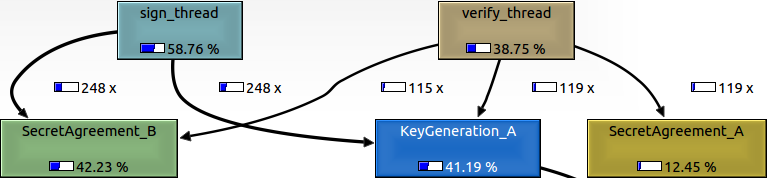
\includegraphics[scale=0.5]{signandverifycall} % e.g. insert ./image for image.png in the working directory, adjust scale as necessary
\caption{<Caption here>}
\label{fig:label} % insert suitable label, this is used to refer to a fig from within the text as shown above
\end{figure}

\subsection{Security Concerns}

Recall the notion of a general side-channel attack: A side-channel attack is performed when an unauthorized individual is able to acquire information by measuring properties of the physical implementation of the system at hand. This can be done by analyzing the power consumption, timing properties, or electromagnetic leaks of a CPU while it operates on (or generates) confidential information.

In the context of information security, algorithms for performing operations over mathematical objects can be said to fall under one of two categories: \emph{constant time} and \emph{non-constant time} algorithms. Constant time algorithms are designed to protect confidential information from side-channel attacks, but come at the cost of computational efficiency.

In the \sidh library, there are two distinct functions for computing field element inversions: \code{fp2inv751\_mont} and \code{fp2inv751\_mont\_bingcd}. \code{fp2inv751\_mont\_bingcd} performs inversion by means of the binary GCD (greatest common denominator) algorithm, and is a \emph{non-constant time} implementation. \code{fp2inv751\_mont} is a \emph{constant time} implementation, and as such runs slower than \code{fp2inv751\_mont\_bingcd} in nearly all cases, but protects against timing based side-channel attacks. They perform comparatively as such:

\begin{center}
\begin{tabular}{@{}lllll@{}}
	\toprule
	Procedure & Performance in clock cyckes & System A With Batching\\
	\midrule
	\code{fp2inv751\_mont} & 68,881,331 & 68,881,331\\
	\code{fp2inv751\_mont\_bingcd} & 15,744,477,032 & 15,565,738,003\\
	\bottomrule
\end{tabular}
\end{center}

Take for example some private data $c$ being manipulated or operated on by some algorithm $\textbf{A}$. In order to be entirely certain that $c$ in \textbf{P($c$)} is not vulnerable to \emph{any} imagineable side-channel attack it must be the case that the structure of \textbf{P} does not in anyway depend on the information stored in $c$.

Let us look more closely at the elements that are inverted by \code{pb\_inv}. In \code{KeyGeneration\_A} the elements being passed to \code{pb\_inv} are simply the constituents of \randall's public key for every iteration of the signing procedure. Because the data being operated on is publicly available information, we needn't consider if it is vulnerable to side-channel analysis. 

In \code{SecretAgreement\_A}, \code{pb\_inv} is called by \code{j\_inv}, which produces the \emph{j}-invariant of a particular curve. When \code{SecretAgreement\_A} is used in the context of SIDH key exchange, \code{j\_inv} is used to compute the shared secret between party members \ba and \rb, and so would need to be protected against side-channel attacks. This is not the case in the context of signatures, however. Recall the structure of SIDH signatures: every signature includes, for every $2\lambda$ iterations, the commitment $E_1$, which is precisely the shared secret between the signer and \randall. And so, every use of \code{pb\_inv} \emph{in the context of signatures} does not require extra precautions to side-channel analysis. The same is true for \code{SecretAgreement\_B}.

While it is not the case for our implementations that the data on which \code{pb\_inv} operates would find itself the subject of side-channel analysis, it is not difficult to imagine a scenario where this might be the case. 


\section{Results}

\begin{center}
\begin{tabular}{@{}llll@{}}
	\toprule
	Modulus Size & Regular Batch & Partial Batched Inversion & Unbatched \\
	\midrule
	32 Inversion & 0.033685 & 0.00080204\\
	64 Inversion & 0.00033685 & 0.00080204\\
	128 Inversion & 0.00033685 & 0.00080204\\
	256 Inversion & 0.00033685 & 0.00080204\\
	512 Inversion & 0.00033685 & 0.00080204\\
	1024 Inversion & 0.00033685 & 0.00080204\\
	2048 Inversion & 0.00033685 & 0.00080204\\
	\bottomrule
\end{tabular}
\end{center}

\begin{center}
\begin{tabular}{@{}llll@{}}
	\toprule
	Modulus Size & Regular Batch & Partial Batched Inversion & Unbatched \\
	\midrule
	32 & 0.00033685 & 0.00080204\\
	64 & 0.00033685 & 0.00080204\\
	128 & 0.00033685 & 0.00080204\\
	256 & 0.00033685 & 0.00080204\\
	512 & 0.00033685 & 0.00080204\\
	1024 & 0.00033685 & 0.00080204\\
	2048 & 0.00033685 & 0.00080204\\
	\bottomrule
\end{tabular}
\end{center}

\begin{center}
\begin{tabular}{@{}llll@{}}
	\toprule
	Modulus Size & Regular Batch & Partial Batched Inversion & Unbatched \\
	\midrule
	32 & 0.00033685 & 0.00080204\\
	64 & 0.00033685 & 0.00080204\\
	128 & 0.00033685 & 0.00080204\\
	256 & 0.00033685 & 0.00080204\\
	512 & 0.00033685 & 0.00080204\\
	1024 & 0.00033685 & 0.00080204\\
	2048 & 0.00033685 & 0.00080204\\
	\bottomrule
\end{tabular}
\end{center}

Two different machines were used for benchmarking. System A denotes a single-core, 1.70 GHz Intel Celeron CPU. System B denotes a quad-core, 3.1 GHz AMD A8-7600.\\

The two figures below provide benchmarks for KeyGen, Sign, and Verify procedures with both batched partial inversion implemented (in the previously mentioned locations) and not implemented. All benchmarks are averages computed from 100 randomized sample runs. All results are measured in clock cycles.

\begin{center}
\begin{tabular}{@{}lllll@{}}
	\toprule
	Procedure & System A Without Batching & System A With Batching\\
	\midrule
	KeyGen & 68,881,331 & 68,881,331\\
	Signature Sign & 15,744,477,032 & 15,565,738,003\\
	Signature Verify & 11,183,112,648 & 10,800,158,871\\
	\bottomrule
\end{tabular}
\end{center}

\begin{center}
\begin{tabular}{@{}lllll@{}}
	\toprule
	Procedure & System B Without Batching & System B With Batching\\
	\midrule
	KeyGen & 84,499,270 & 84,499,270\\
	Signature Sign & 10,227,466,210 & 10,134,441,024\\
	Signature Verify & 7,268,804,442 & 7,106,663,106\\
	\bottomrule
\end{tabular}
\end{center}

\textbf{System A:} With inversion batching turned on we notice a ~1.1 \% performance increase for key signing and a ~3.5 \% performance increase for key verification.\\

\textbf{System B:} With inversion batching turned on we a observe a ~0.9 \% performance increase for key signing and a ~2.3 \% performance increase for key verification.\\

\subsection{Analysis}

It should first be noted that, because our benchmarks are measured in terms of clock cycles, the difference between our two system clock speeds should be essentially ineffective. \\

In the following table, ``Batched Inversion" signifies running \code{pb\_inv} on 248 $\mathbb{F}_{p^{2}}$ elements.

\begin{center}
\begin{tabular}{@{}ll@{}}
	\toprule
	Procedure & Performance \\
	\midrule
	Batched Inversion & 1721718\\
	$\mathbb{F}_{p^{2}}$ Montgomery Inversion & 874178\\
	\bottomrule
\end{tabular}
\end{center}

The following are all measured in clock cycles, as the computed average of 1000 distinct executions:

\begin{center}
\begin{tabular}{@{}lll@{}}
	\toprule
	Modulus Size & Multiplication & Inversion Time \\
	\midrule
	32 & 0.00033685 & 0.00080204\\
	64 & 0.00033685 & 0.00080204\\
	128 & 0.00033685 & 0.00080204\\
	256 & 0.00033685 & 0.00080204\\
	512 & 0.00033685 & 0.00080204\\
	1024 & 0.00033685 & 0.00080204\\
	2048 & 0.00033685 & 0.00080204\\
	\bottomrule
\end{tabular}
\end{center}

Do performance increases observed make sense?\\

\subsection{Remaining Opportunities}
There are two functions called in the isogeny signature system that perform a $\mathbb{F}_{p^{2}}$ inversion: \code{j\_inv} and \code{inv\_4\_way}. These functions are called once in SecretAgreement and KeyGeneration operations respectively. SecretAgreement and KeyGeneration are in turn called from each signing and verification thread.

This means that in the signing procedure there are 2 opportunities for implementing batched partial-inversion with a batch size of 248 elements. In the verify procedure, however, there are 3 opportunities for implementing batched inversion with a batch size of roughly ~124 elements.

Another avenue for implementation of this procedure, much in line with Fiat's original RSA batch, lies in . We discuss this approach in greater detail in section \ref{sec:morebatch}.
